\begin{pages}
    \begin{Rightside}
    \selectlanguage{greek}
        \beginnumbering
        \pstart[
        			\chapter{Τὸ τοὺς πρώτους ἀγγέλους σαλπίσαι}
        			\markboth{The Sounding of the First Angels}
				]
		Καὶ ὅταν ἤνοιξεν τὴν σφραγῖδα τὴν ἑβδόμην, ἐγένετο σιγὴ ἐν τῷ οὐρανῷ ὡς ἡμιώριον. καὶ εἶδον τοὺς ἑπτὰ ἀγγέλους οἳ ἐνώπιον τοῦ Θεοῦ ἑστήκασιν, καὶ ἐδόθησαν αὐτοῖς ἑπτὰ σάλπιγγες. Καὶ ἄλλος ἄγγελος ἦλθεν καὶ ἐστάθη ἐπὶ τοῦ θυσιαστηρίου ἔχων λιβανωτὸν χρυσοῦν, καὶ ἐδόθη αὐτῷ θυμιάματα πολλὰ ἵνα δώσει ταῖς προσευχαῖς τῶν ἁγίων πάντων ἐπὶ τὸ θυσιαστήριον τὸ χρυσοῦν τὸ ἐνώπιον τοῦ θρόνου. 
		\pend
		\pstart
		καὶ ἀνέβη ὁ καπνὸς τῶν θυμιαμάτων ταῖς προσευχαῖς τῶν ἁγίων ἐκ χειρὸς τοῦ ἀγγέλου ἐνώπιον τοῦ Θεοῦ. καὶ εἴληφεν ὁ ἄγγελος τὸν λιβανωτόν, καὶ ἐγέμισεν αὐτὸν ἐκ τοῦ πυρὸς τοῦ θυσιαστηρίου καὶ ἔβαλεν εἰς τὴν γῆν· καὶ ἐγένοντο βρονταὶ καὶ φωναὶ καὶ ἀστραπαὶ καὶ σεισμός. Καὶ οἱ ἑπτὰ ἄγγελοι οἱ ἔχοντες τὰς ἑπτὰ σάλπιγγας ἡτοίμασαν αὑτοὺς ἵνα σαλπίσωσιν.
		\pend
		\pstart
		Καὶ ὁ πρῶτος ἐσάλπισεν· καὶ ἐγένετο χάλαζα καὶ πῦρ μεμιγμένα ἐν αἵματι καὶ ἐβλήθη εἰς τὴν γῆν· καὶ τὸ τρίτον τῆς γῆς κατεκάη, καὶ τὸ τρίτον τῶν δένδρων κατεκάη, καὶ πᾶς χόρτος χλωρὸς κατεκάη. 
		\pend
		\pstart
		Καὶ ὁ δεύτερος ἄγγελος ἐσάλπισεν· καὶ ὡς ὄρος μέγα πυρὶ καιόμενον ἐβλήθη εἰς τὴν θάλασσαν· καὶ ἐγένετο τὸ τρίτον τῆς θαλάσσης αἷμα, καὶ ἀπέθανεν τὸ τρίτον τῶν κτισμάτων τῶν ἐν τῇ θαλάσσῃ, τὰ ἔχοντα ψυχάς, καὶ τὸ τρίτον τῶν πλοίων διεφθάρησαν. 
		\pend
		\pstart
		Καὶ ὁ τρίτος ἄγγελος ἐσάλπισεν· καὶ ἔπεσεν ἐκ τοῦ οὐρανοῦ ἀστὴρ μέγας καιόμενος ὡς λαμπάς, καὶ ἔπεσεν ἐπὶ τὸ τρίτον τῶν ποταμῶν καὶ ἐπὶ τὰς πηγὰς τῶν ὑδάτων. καὶ τὸ ὄνομα τοῦ ἀστέρος λέγεται Ὁ Ἄψινθος. καὶ ἐγένετο τὸ τρίτον τῶν ὑδάτων εἰς ἄψινθον, καὶ πολλοὶ τῶν ἀνθρώπων ἀπέθανον ἐκ τῶν ὑδάτων ὅτι ἐπικράνθησαν. 
		\pend
		\pstart
		Καὶ ὁ τέταρτος ἄγγελος ἐσάλπισεν· καὶ ἐπλήγη τὸ τρίτον τοῦ ἡλίου καὶ τὸ τρίτον τῆς σελήνης καὶ τὸ τρίτον τῶν ἀστέρων, ἵνα σκοτισθῇ τὸ τρίτον αὐτῶν καὶ ἡ ἡμέρα μὴ φάνῃ τὸ τρίτον αὐτῆς, καὶ ἡ νὺξ ὁμοίως. Καὶ εἶδον, καὶ ἤκουσα ἑνὸς ἀετοῦ πετομένου ἐν μεσουρανήματι λέγοντος φωνῇ μεγάλῃ Οὐαὶ οὐαὶ οὐαὶ τοὺς κατοικοῦντας ἐπὶ τῆς γῆς ἐκ τῶν λοιπῶν φωνῶν τῆς σάλπιγγος τῶν τριῶν ἀγγέλων τῶν μελλόντων σαλπίζειν.
		\pend
        \endnumbering
    \end{Rightside}
    \begin{Leftside}
        \beginnumbering
        \pstart[
        			\chapter{The Sounding of \\ the First Angels}
				]
		And when He (the Lamb) opened the seventh seal, a great silence occurred, (lasting for) approximately half an hour. And I saw the seven angels — (namely) those which were standing before God — and they were given seven trumpets. And another angel came and stood upon the altar (whilst) having a golden censer (in his hand); and plenty of incense was given to him so that he may give it with the prayers of all the holy men upon the golden altar, (namely the one) before the throne.
		\pend
		\pstart
		And the smoke of the incense arose with the prayers of the holy men, (left the) hand of the angel and (went up) before God. And the angel took the censer and filled it from (with) the fire of the altar and took it to the Earth. And there were thunders and voices and lightnings and a tremor. And the seven angels — the ones who have the seven trumpets — prepared themselves so that they might (begin) sounding (the trumpets). 
		\pend
		\pstart
		And the first (one) sounded (his trumpet). And there was hail and fire mixed with blood and it was thrown into (onto) the Earth; and a third of the Earth was burnt (down), and a third of the trees were burnt (down) and every (bit) of green grass was burnt (down).
		\pend
		\pstart
		And the second angel sounded (his trumpet). And (something that was) like a great, fiery mountain was hurled into the sea. And a third of the sea became blood, and a third of the creatures of the sea — namely those who live in the sea and have a soul (who are alive) — died; and a third of the ships were destroyed. 
		\pend
		\pstart
		And the third angel sounded (his trumpet). And (there) fell from (the) Heaven a great star, burning like a torch; and it fell into (upon) a third of the rivers and into (upon) the springs of waters. And the name of the star is Wormwood (Apsinthos). And a third of the waters became wormwood and many (of the) humans died because of the waters, because they were made bitter. 
		\pend
		\pstart
		And the fourth angel sounded (his trumpet). And a third of the Sun was struck, and a third of the Moon and a third of the stars, so that a third of them was darkened (shadowed) and (so that) the day — as well as night — does not shine (upon) a third of them. And I saw and I heard an eagle flying in mid-air saying, “Woe, woe, woe to those who live upon the Earth from the remaining trumpet voices of the three angels that are about to sound (their trumpets). 
		\pend
        \endnumbering
    \end{Leftside}

\end{pages} 
\Pages

\clearpage
\thispagestyle{empty}
\null\vfill
\settowidth\longest{\huge\itshape […] and when I turned around I saw}
\begin{center}
\parbox{\longest}{%
  \raggedright{\huge\itshape%
    ``And when He (the Lamb) opened the seventh seal, a great silence occurred, (lasting for) approximately half an hour.'' \par\bigskip
  }
  \raggedleft\Large\MakeUppercase{``Opening of the Seventh Seal'' — John Martin, 1837}\par%
}
\vfill\vfill
\clearpage\newpage
\end{center}
\newpage
\thispagestyle{empty}
\begin{center}
	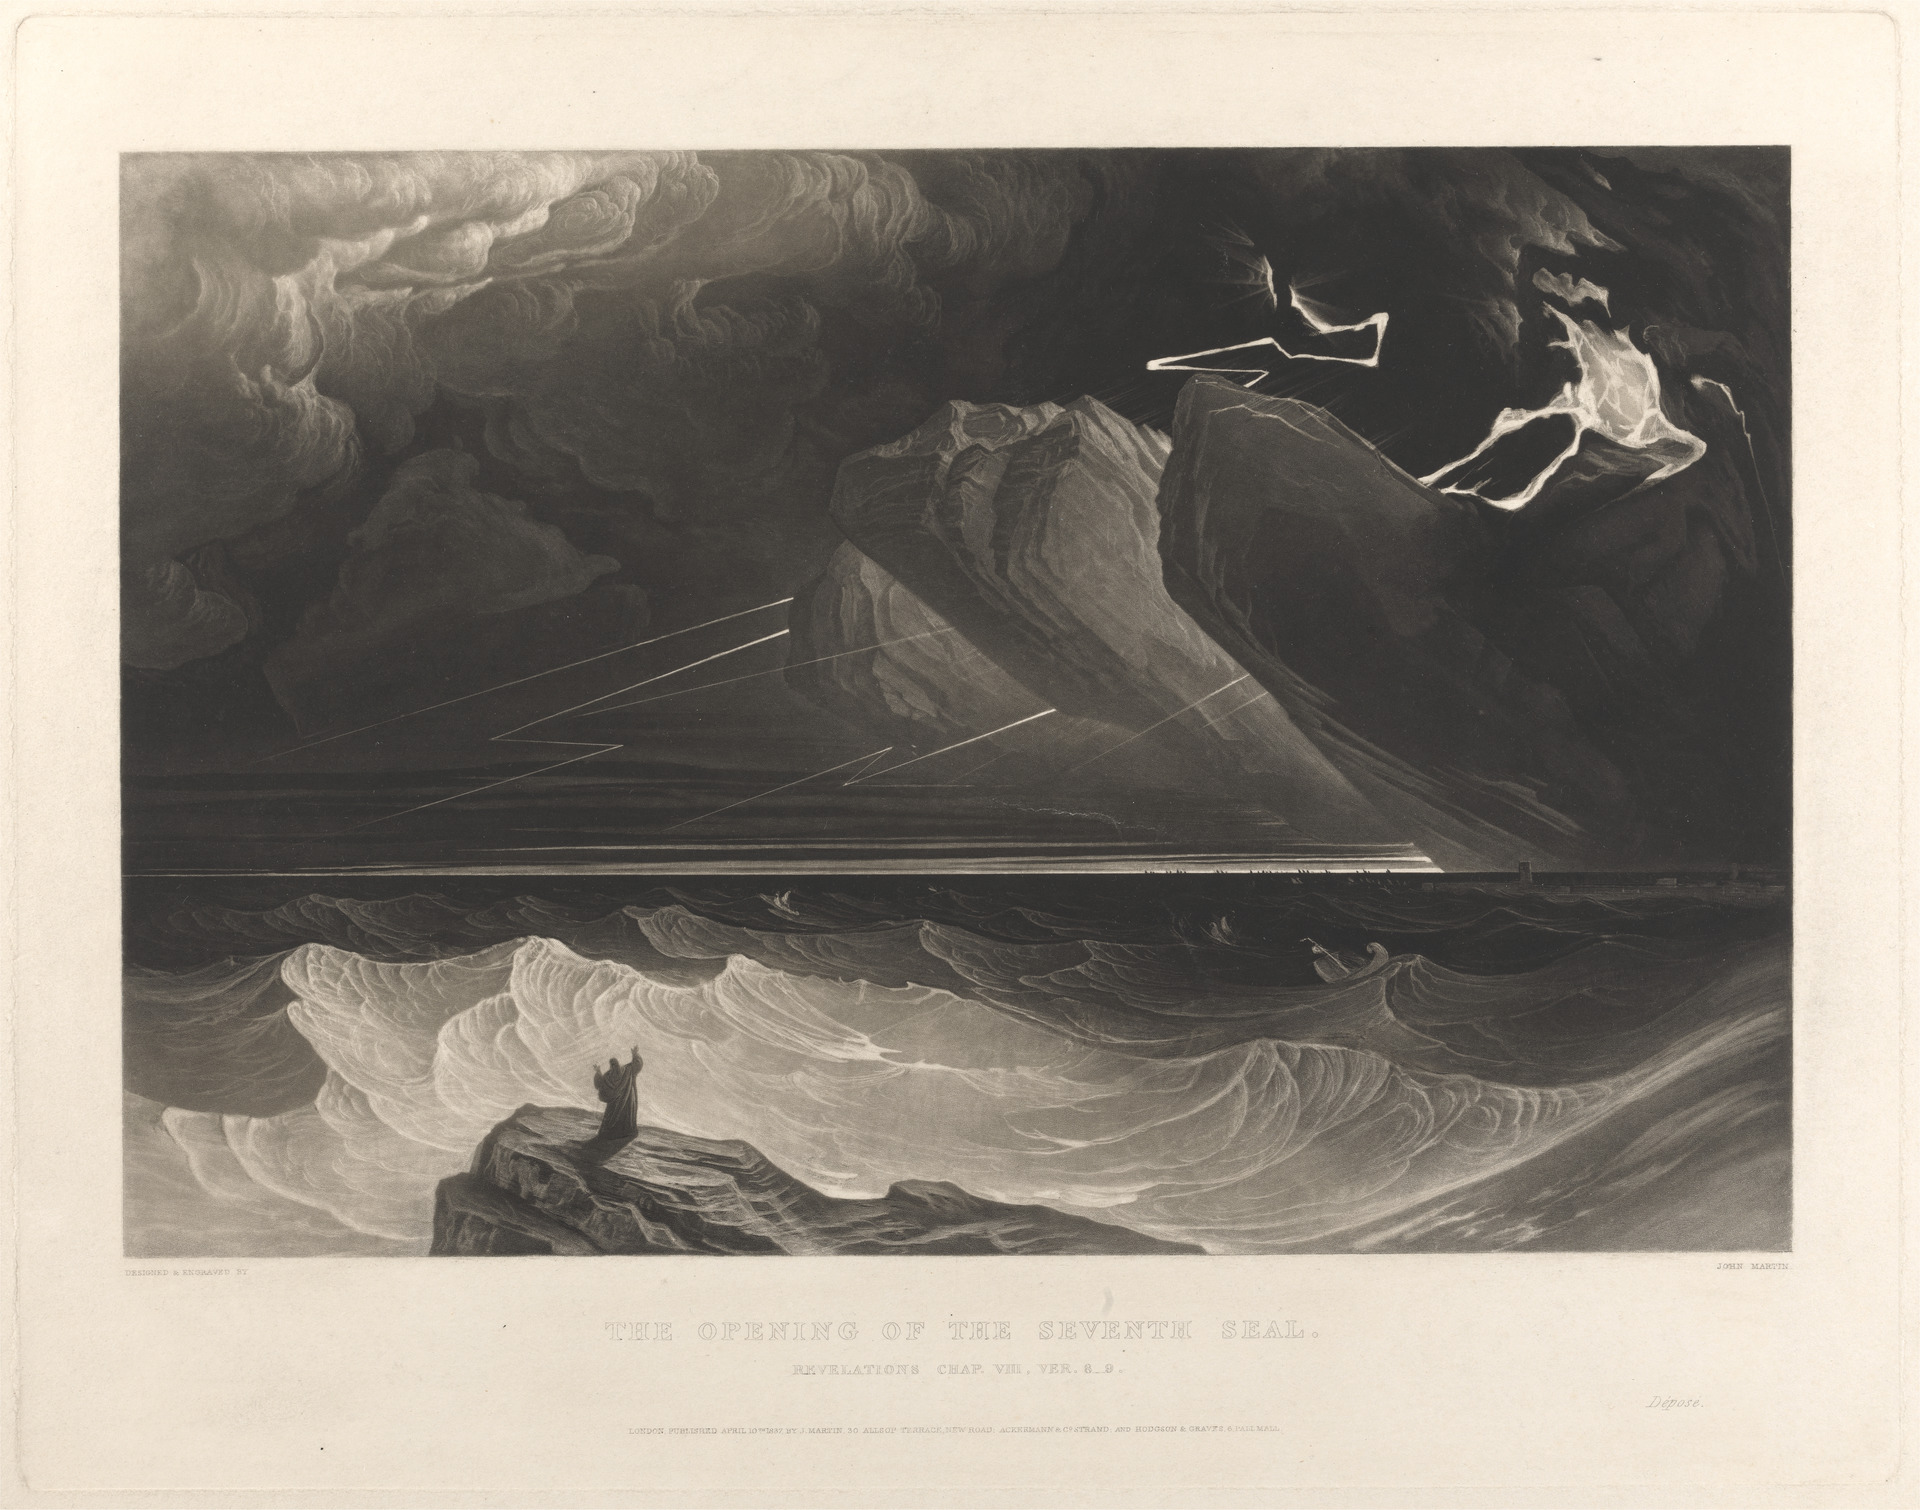
\includegraphics[angle=90, width=1\textwidth]{images/illustrations/johnmartinseventhseal.jpg}
\end{center}